%%%%%%%%%%%%%%%%%%%%%%%%%%%%%%%%%%
%% E V I C T I N G    B L O C K %%
%%%%%%%%%%%%%%%%%%%%%%%%%%%%%%%%%%

\subsection{Evicting Block}
\label{subsec:evicting_block}

The Evicting Block is responsible for selecting a victim way when a cache miss occurs and a new cache line has to be allocated. The module implements the \textit{Not Most Recently Used} (NMRU) replacement policy.

\begin{figure}[h]
	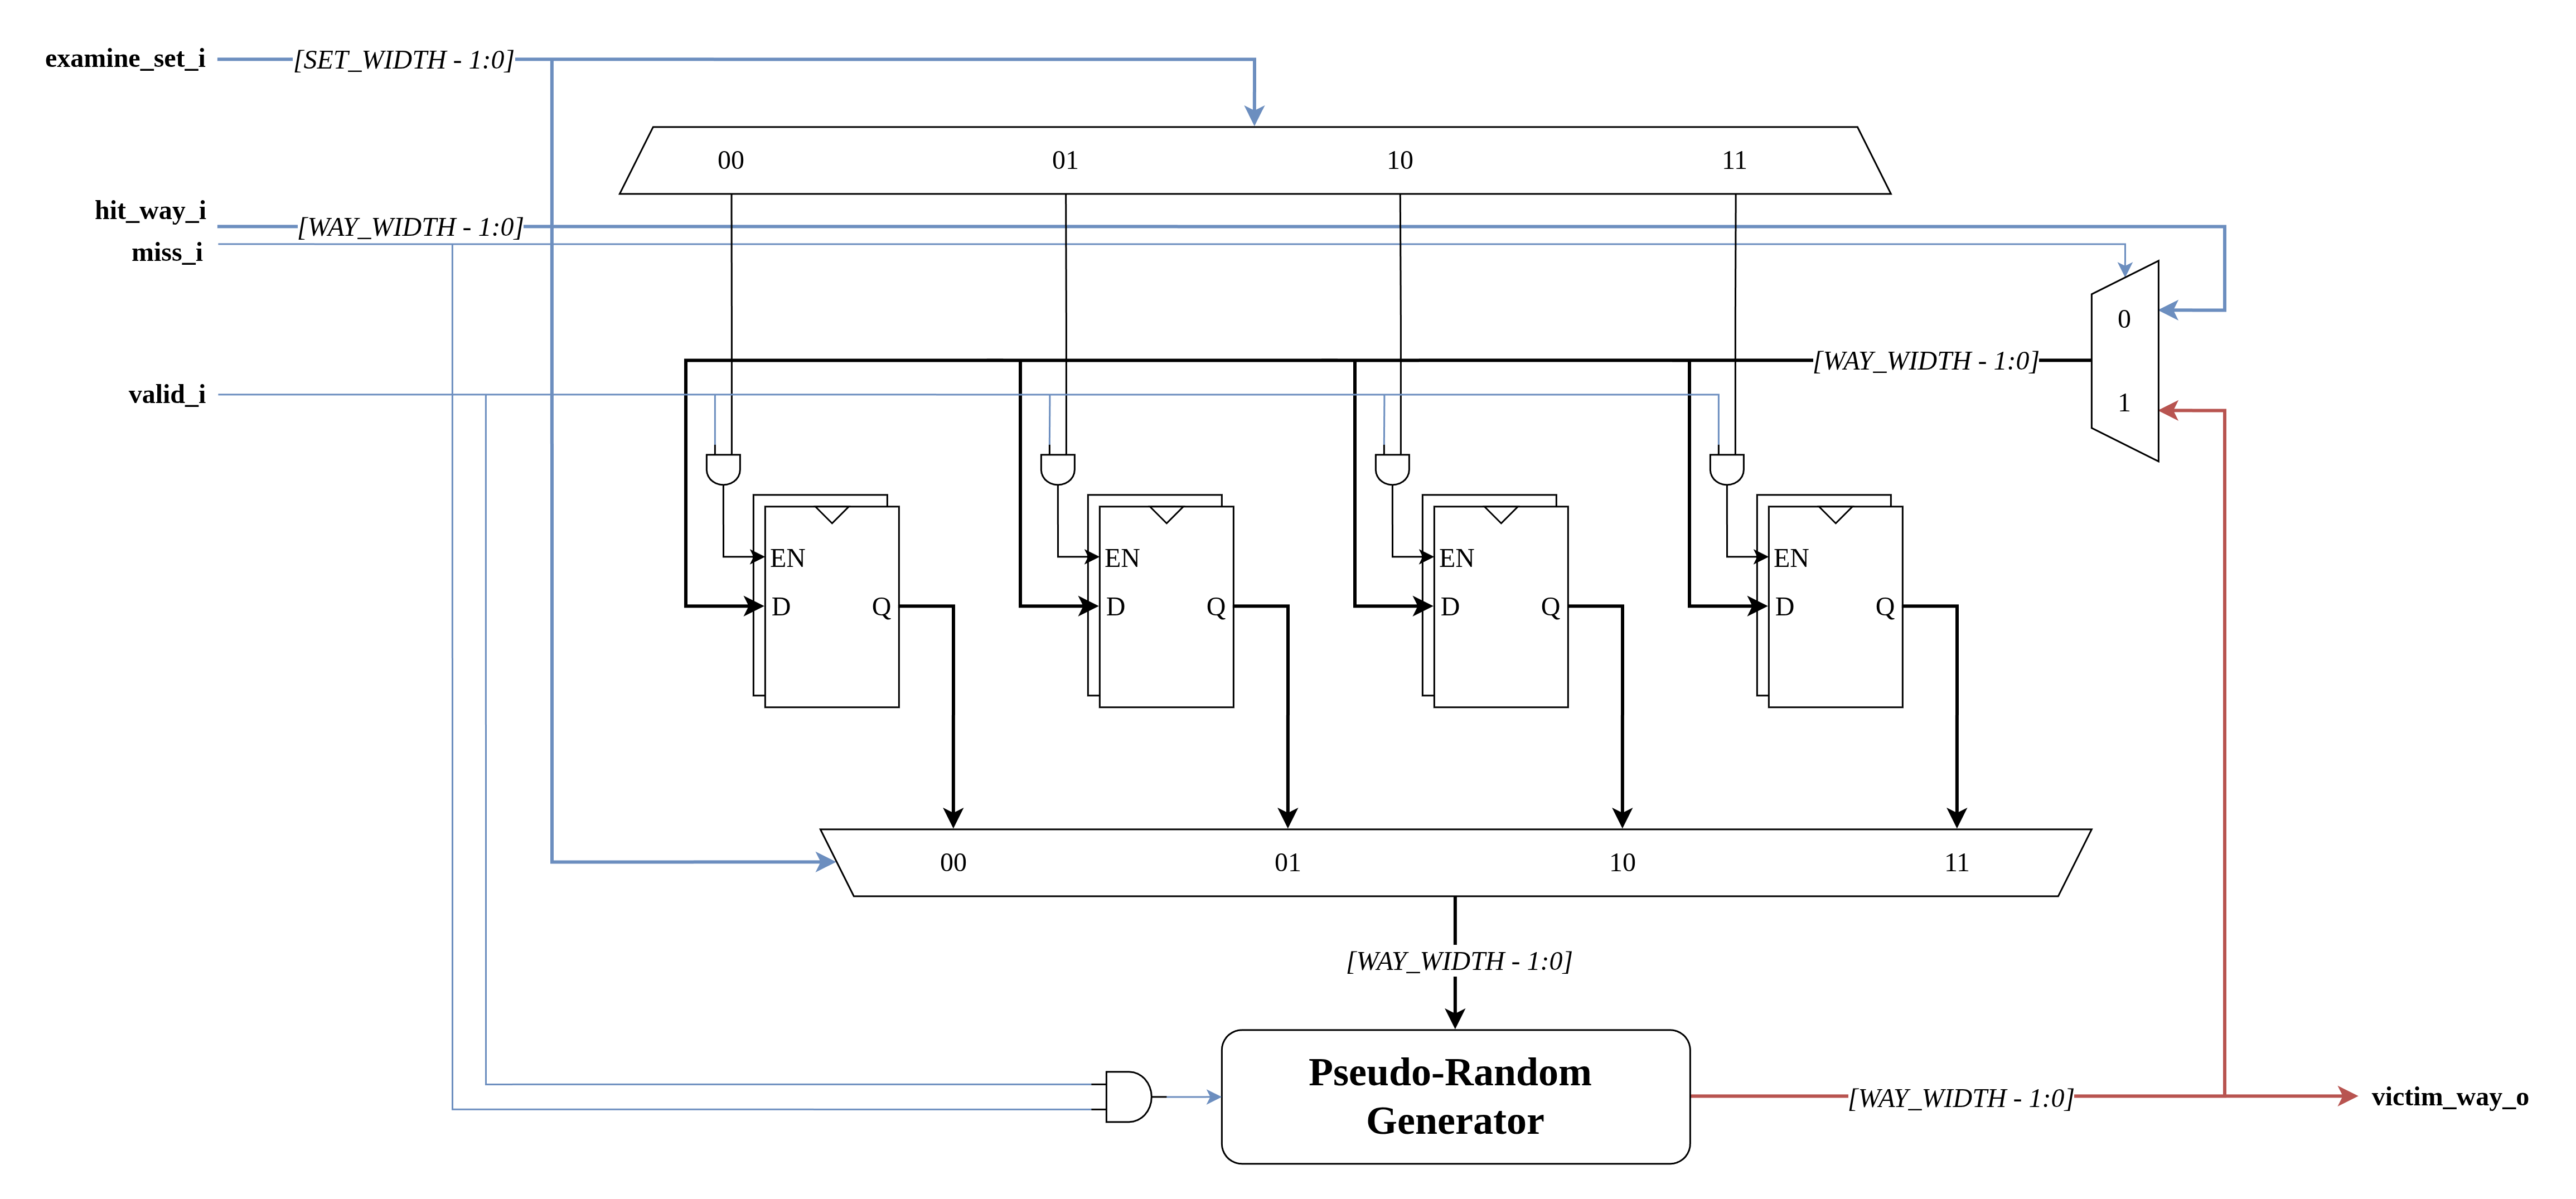
\includegraphics[width=16cm]{NMRU.png}
	\caption{Evicting Block scheme (4-set cache)}
\end{figure}

\begin{table}[htbp]
	\centering
	\small
	\begin{tabularx}{\textwidth}{l c c X}
		\toprule
		\textbf{Parameter} & \textbf{Valid Range} & \textbf{Default} & \textbf{Description} \\
		\midrule
		
		\verb|SET_NUM| &
		Positive integer &
		--- &
		Number of cache sets for which the replacement state is maintained. \\
		
		\verb|WAY_NUM| &
		Positive integer &
		--- &
		Number of cache ways used for victim selection. \\
		
		\bottomrule
	\end{tabularx}
	\caption{Evicting Block parameters}
	\label{tab:evicting_block_parameters}
\end{table}

\begin{table}[htbp]
	\centering
	\label{tab:evicting_block_ports}
	\small
	\begin{tabularx}{\textwidth}{l c c X}
		\toprule
		\textbf{Ports} & \textbf{Direction} & \textbf{Width} & \textbf{Description} \\
		\midrule
		\verb| examine_set_i | & Input & \verb| SET_WIDTH | & Index of the current cache set. \\
		\verb| hit_way_i | & Input & \verb| WAY_WIDTH | & Index of the way containing the requested tag on a cache hit. \\
		\verb| miss_i | & Input & \verb| 1 | & Indicates that the current cache access resulted in a cache miss. \\
		\verb| valid_i | & Input & \verb| 1 | & Indicates whether the selected cache line contains valid data. \\
		\verb| victim_way_o | & Output & \verb| WAY_WIDTH | & Index of the way selected for replacement on a cache miss. \\
		\bottomrule
	\end{tabularx}
	\caption{Evicting Block ports}
\end{table}

The module maintains a separate register for each cache set. Each register stores the index of the way that was most recently used within the corresponding set.

When a cache access results in a hit, the way containing the requested tag becomes the most recently used way.

When a cache miss occurs, the module receives the index of the selected set and reads the corresponding MRU (Most Recently Used) register. The stored way index is then used as a constraint for victim selection: the victim way must not be equal to the most recently used way.

To select the victim, the module contains a \PRG. The generator is activated on a cache miss and produces a candidate way index.

Once a valid victim way has been generated, its index is driven to the module output and is used by the cache control logic to select the way that will be replaced. The selected victim way also becomes the new most recently used way. Therefore, the current MRU register is updated with the generated victim index. This ensures that the most recently accessed or allocated way is excluded from being selected as the victim during the next replacement operation for the same set.